\chapter{Example of a GTK+ Application Code Architecture}
\label{gtk-app-arch}

%FIXME: re-explain what is a "widget" and "container". And add a glossary at the end.

For any programming project, it is important to design correctly the general code architecture. With Object-Oriented Programming, it means defining the main classes. This chapter explains one good example of a code architecture for a GTK+ application, by looking at a simplified view of the gedit text editor\footnote{\url{https://wiki.gnome.org/Apps/Gedit}}.

gedit has a tabbed document interface: several files can be opened in the same gedit window, in different tabs. As we will see, this is reflected in the code architecture.

The Figure~\ref{fig:gedit-architecture} p.~\pageref{fig:gedit-architecture} shows the class schema. Every gedit class in the schema is a subclass of a GTK+ or GtkSourceView class. (GtkSourceView\footnote{\url{https://wiki.gnome.org/Projects/GtkSourceView}} is a library extending the \lstinline{GtkTextView} widget; \lstinline{GtkTextView} being part of GTK+.)

We will go through the class schema, explaining the classes step by step, by beginning at the top. This will permit to introduce some of the most important GTK+ classes, not by describing them in details with a lot of code examples, but by giving a high-level overview.

\begin{figure}
  \begin{center}
    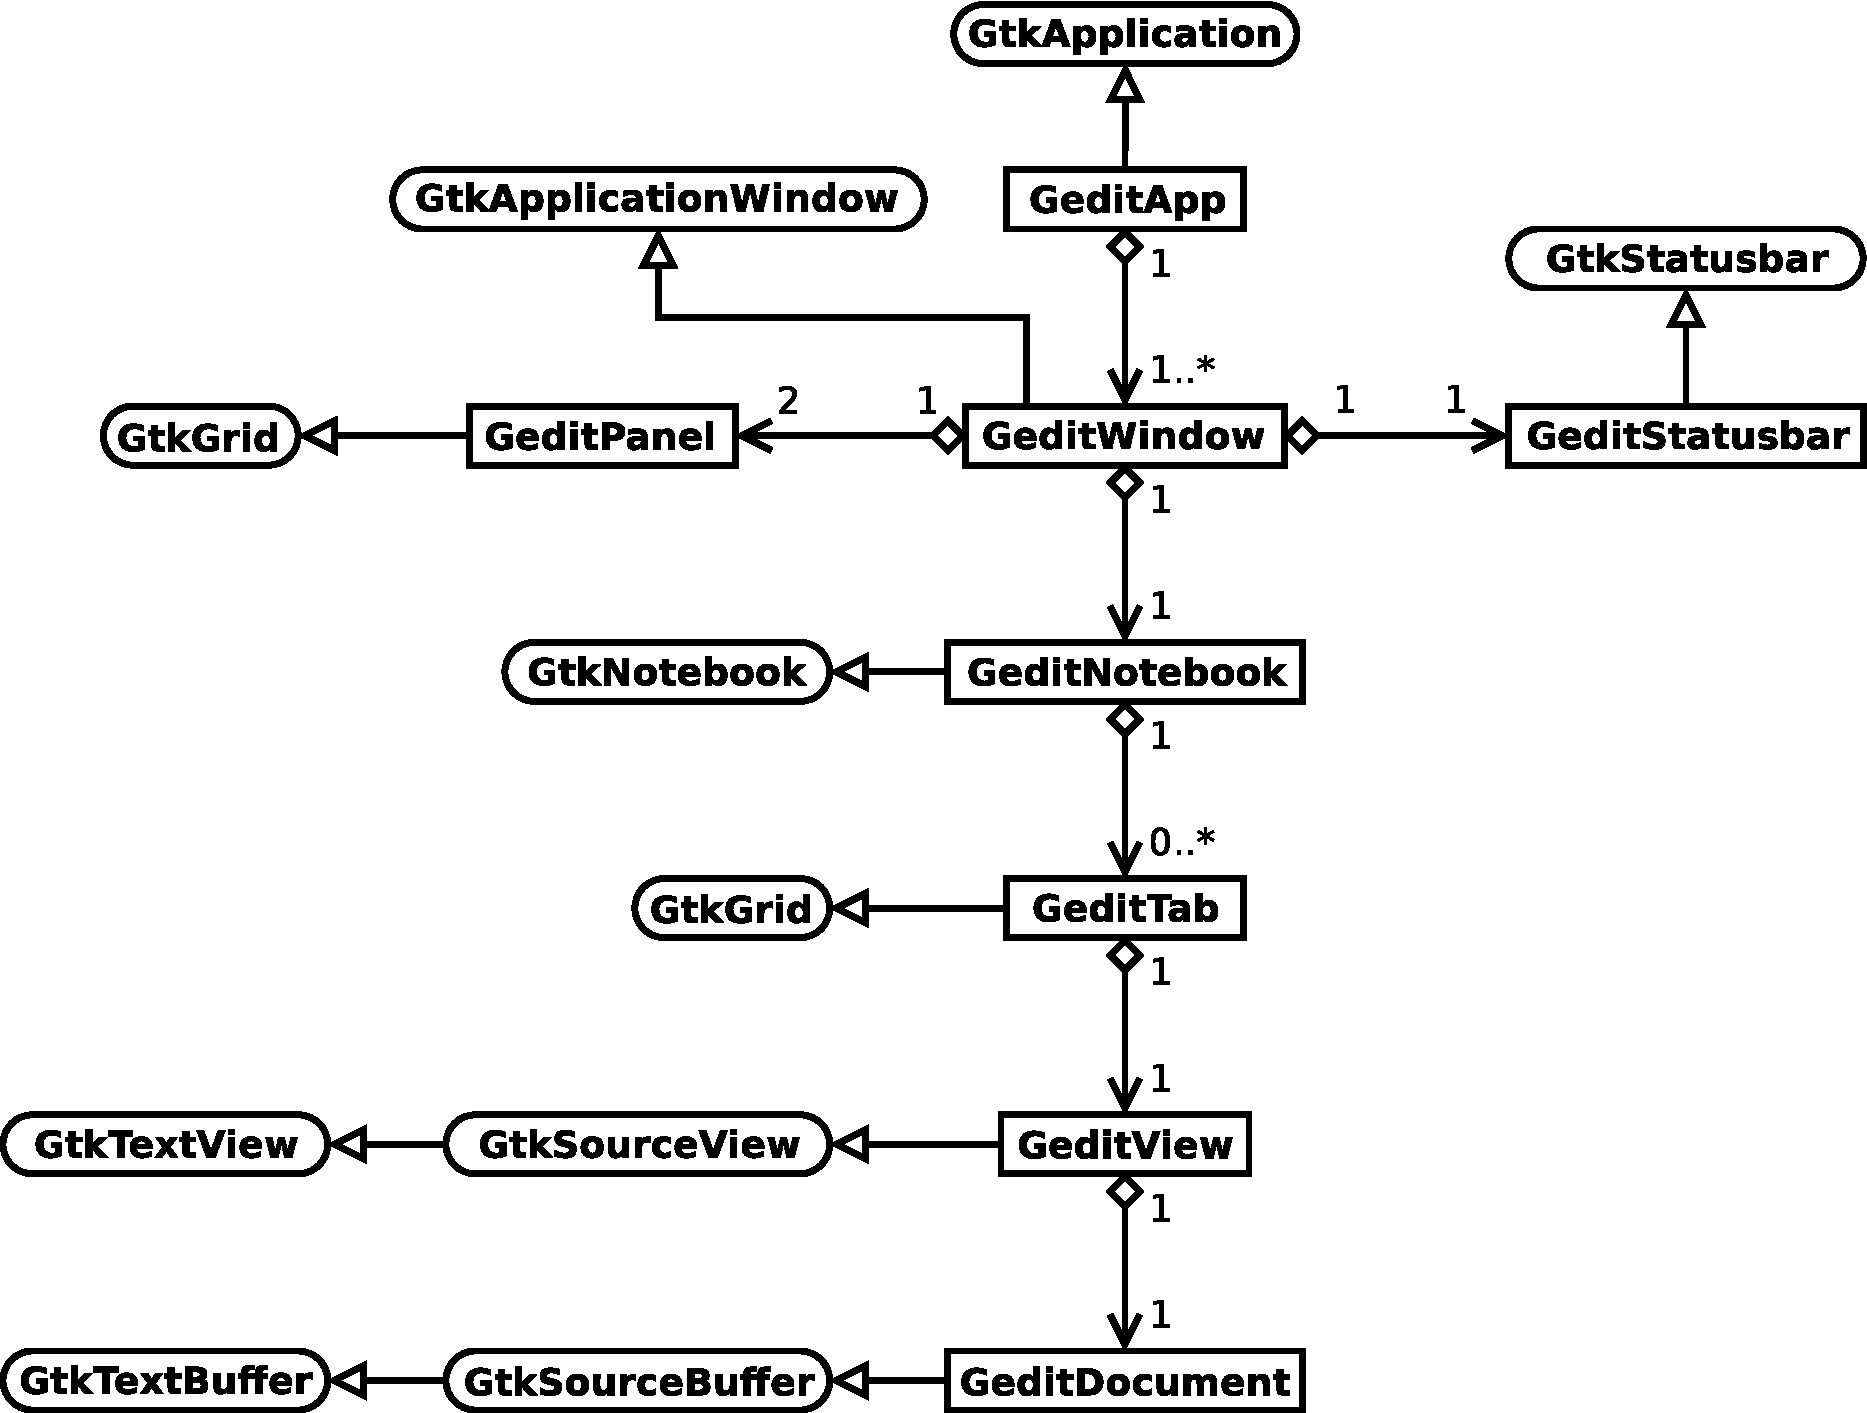
\includegraphics[width=\textwidth]{images/gedit-architecture.pdf}
    \caption{Simplified code architecture of the gedit text editor}
    \label{fig:gedit-architecture}
  \end{center}
\end{figure}

\section{The main() function and GeditApp}

Although not represented on the schema, the entry point of a GTK+ application --~as for every C program~-- is the \lstinline{main()} function. To create a GTK+ application, the principal thing to do in \lstinline{main()} is to create a \lstinline{GtkApplication} instance, or a subclass of it. In the schema we see that \lstinline{GeditApp} is a subclass of \lstinline{GtkApplication}, so the \lstinline{main()} function of gedit creates a \lstinline{GeditApp} object.

\lstinline{GtkApplication} is the class that contains and represents the whole application. There is usually only one instance of \lstinline{GtkApplication} per process, so it can be considered a singleton class. What \lstinline{GtkApplication} contains are the \emph{windows}, for example the \lstinline{GeditWindow}'s in case of gedit, plus other types of windows like dialog windows.

We already saw the \lstinline{GtkApplication} class hierarchy in section~\ref{oop-gobject-inheritance} p.~\pageref{oop-gobject-inheritance} when explaining OOP inheritance with GObject:

\begin{verbatim}
GObject
└── GApplication
    └── GtkApplication
\end{verbatim}

\lstinline{GApplication} is part of the GIO library and implements the features that are not related to the Graphical User Interface (GUI). So for a program that runs in the terminal, it is possible to use \lstinline{GApplication} only.

An important feature that \lstinline{GApplication} provides is process uniqueness (but it can be disabled if not wanted). What process uniqueness does is to have only one process per application per user session. For that feature to work, an application ID must be provided when creating the \lstinline{GApplication} object. With that ID, \lstinline{GApplication} looks if another process already runs the same application in the same user session; if it is the case, it communicates to the primary instance the actions that need to be done (for example opening a new window, or opening a new file in an existing window, etc). When the actions are done on the primary instance, the second process exits immediately. On Linux, \lstinline{GApplication} uses the D-Bus Inter-Process Communication (IPC) system to communicate between the two processes.

Process uniqueness has several advantages, to give a few concrete examples:
\begin{itemize}
  \item For an application with a tabbed document interface, when clicking on a file in a file manager like Nautilus, the file can be opened in a new tab instead of creating each time a new window. For this to work, inter-process communication is needed in one form or another;
  \item An application doesn't need to synchronize explicitly its state and data between different processes. For the sake of argument, let's say that in gedit the user can create custom ``build tools'', to compile the current file or project. gedit saves the custom build tools in an XML file and are shown in the menu to execute their commands. On Linux, the XML file is saved for example in the user's \texttt{\textasciitilde{}/.local/share/} directory. Without process uniqueness, if one gedit process modifies the custom build tools, the other gedit processes need to reload the XML file, and need to ensure that there are no races (two different gedit processes must not modify the XML file at the same time). With process uniqueness, that problem doesn't exist, all the gedit windows share the same application state, and the developer can assume that only one process per user can modify the XML file\footnote{Note that this would not be true if it was possible to open \emph{several} graphical sessions for the same user, on the same machine (with multi-seat support) or at least sharing the backing storage for the home directory (for example with NFS mounts). But GNOME and most applications don't support this, a user can open at most one graphical session at a time for the same home directory. For logins on the same physical machine, this is enforced by GDM (the GNOME display manager and login screen) and D-Bus. For NFS mounts this is not enforced, but if the same user opens several graphical sessions on different computers, some programs might misbehave. So although the \lstinline{GApplication} process uniqueness is documented as being per \emph{user session}, in practice we can say that it is simply per \emph{user}.} (of course the user has still the possibility to edit the XML file by hand, but in that case the application can just be restarted, normally the user is expected to modify the build tools from the GUI that gedit provides).
\end{itemize}

Another important feature of \lstinline{GApplication} is to run the main event loop. The GLib main event loop was described in section~\ref{glib-main-event-loop} p.~\pageref{glib-main-event-loop}. With \lstinline{GApplication}, this is done with the \lstinline{g_application_run()} function. A minimalistic version of the \lstinline{main()} function in gedit would look like:

\begin{lstlisting}
int
main (int    argc,
      char **argv)
{
  GeditApp *app;
  int status;

  /* Init i18n (internationalization) here. */

  app = gedit_app_new ();
  status = g_application_run (G_APPLICATION (app), argc, argv);
  g_object_unref (app);

  return status;
}
\end{lstlisting}

What \lstinline{GeditApp} does is basically what would need to be done in \lstinline{main()} if there was no \lstinline{GtkApplication} subclass. This includes:
\begin{itemize}
  \item Configuring the \lstinline{GtkApplication} object correctly, for example giving the application ID;
  \item Connecting callbacks to some signals\footnote{But note that in a GObject subclass, instead of connecting callbacks to signals of a parent class with e.g. \lstinline{g_signal_connect()}, it is better to override the virtual functions instead.}, for example to create a \lstinline{GeditWindow} when needed;
  \item Implementing application-wide \lstinline{GAction}'s. \lstinline{GAction} is a class part of GIO that represents an action that the user can trigger. An application-wide action is for example to quit the application, or to open the preferences dialog (because the preferences are applied to the whole application).
\end{itemize}

When you start writing a new GTK+ application, you don't see directly the need for a \lstinline{GtkApplication} subclass, since the code in \lstinline{main()}, plus the callbacks, are still small. But when more and more features are added, it is a good idea at some point to move the code to a \lstinline{GtkApplication} subclass. Or to create a subclass directly. A subclass is especially useful when the need arises to store additional data.

\section{GeditWindow}

\lstinline{GeditWindow} is a subclass of \lstinline{GtkApplicationWindow}. And, we don't see it on the schema, but \lstinline{GtkApplicationWindow} is a subclass of \lstinline{GtkWindow}, which is a top-level widget. A top-level widget cannot be contained in another widget. A \lstinline{GtkApplicationWindow} is contained in a \lstinline{GtkApplication}, but \lstinline{GtkApplication} is not a subclass of \lstinline{GtkWidget}.

In the schema, the ``\texttt{1}'' and ``\texttt{1..*}'' notation means that one \lstinline{GeditApp} object \emph{contains} one or several \lstinline{GeditWindow} objects, and that a \lstinline{GeditWindow} is contained in exactly one \lstinline{GeditApp} (a \lstinline{GeditWindow} cannot be contained in several \lstinline{GeditApp} objects, there is anyway only one \lstinline{GeditApp} instance per process).

\lstinline{GeditWindow} is responsible to create the main UI, creating other widgets and assembling them in a \lstinline{GtkGrid} container for example. Another thing that \lstinline{GeditWindow} does is to implement the \lstinline{GActions} that have an effect only on the current window, for example an action to close the window, or save the current document. When implementing a \lstinline{GAction}, \lstinline{GeditWindow} can of course delegate most of its work to other classes contained in \lstinline{GeditWindow}.

At the top of a main application window, there is usually a \lstinline{GtkHeaderBar}, that shows the window title, some buttons and an ``hamburger'' menu. Alternatively, an application can have a traditional menubar and toolbar.

Besides the headerbar, \lstinline{GeditWindow} creates a \lstinline{GeditStatusbar} widget and adds it to the bottom of the window. It also creates two \lstinline{GeditPanels}, one on the left side of the window, and the other on the bottom, above the \lstinline{GeditStatusbar}. Each panel can contain several elements. For example the side panel contains an integrated file browser, and the bottom panel can contain a terminal, among other things\footnote{The current gedit code actually doesn't contain a \lstinline{GeditPanel} class anymore, but it was the case in an earlier version. Adding \lstinline{GeditPanel} to the diagram was done to show a possible implementation of panels in an application. If your application contains only one element in a panel, no need to have a \lstinline{Panel} class, you can directly add the element to the window.}.

\lstinline{GeditWindow} also creates a \lstinline{GeditNotebook}, the main part of the window.

\section{GeditNotebook and What It Contains}

\lstinline{GeditNotebook} is a subclass of \lstinline{GtkNotebook}, which is the widget that displays tabs, and also contains their content.

In the class schema, we can see that the content of a tab is a \lstinline{GeditTab} widget, a subclass of \lstinline{GtkGrid}. The main element inside a \lstinline{GeditTab} is the \lstinline{GeditView}. More precisely --- it was omitted in the schema for succinctness --- the \lstinline{GeditView} is actually contained in a \lstinline{GtkScrolledWindow} which is contained in the \lstinline{GeditTab}. But \lstinline{GeditTab} can contain other widgets, for example information bars on top of the document.

\lstinline{GeditView} is a subclass of \lstinline{GtkSourceView}, which is itself a subclass of \lstinline{GtkTextView}. \lstinline{GtkTextView} --- which is part of GTK+ --- is the foundation for a multiline text editor. The GtkSourceView library adds features useful for source code, such as syntax highlighting. \lstinline{GtkTextView} follows a Model-View-Controller pattern. \lstinline{GtkTextBuffer} is the model, i.e. it contains the data.

\section{Why and When Creating Sub-Classes of GTK+ Widgets?}

If we look for instance at \lstinline{GeditTab}, it contains --- by composition --- a \lstinline{GeditView}. \lstinline{GeditView} is a subclass of \lstinline{GtkSourceView}. Instead, \lstinline{GeditTab} could use by composition directly a \lstinline{GtkSourceView} object, and move the code of \lstinline{GeditView} to \lstinline{GeditTab}. But usually, it's exactly the opposite that happens or should happen.

When a GTK+ application codebase is still small, for example if you start writing an equivalent of \lstinline{GeditTab}, you can create a \lstinline{GtkSourceView} object directly in \lstinline{GeditTab}, and store the \lstinline{GtkSourceView} object in an instance variable. Then, when implementing new features, you add new functions that use almost exclusively the \lstinline{GtkSourceView} instance variable. You may even have \lstinline{static} functions that take directly a \lstinline{GtkSourceView} argument instead of the \lstinline{GeditTab} \emph{self} parameter. You may also store additional data useful only to the \lstinline{GtkSourceView}-related functions. If the \lstinline{GeditTab} class is still small (e.g. 500 lines of code) and doesn't contain a lot of instance variables, there is no problem. On the other hand, if the \lstinline{GeditTab} class becomes larger (e.g. more than 2000 lines of code), then it's probably a sign that the class should delegate some of its work to a new class; in our case, \lstinline{GeditView}. Note that 2000 lines of code for a class might be fine, there is no clear boundary on when a class should be split. But if the resulting \lstinline{GeditView} class would contain at least several hundreds of non-boilerplate code, it is probably a good idea to do the refactoring.

What OOP is all about is to pack data and behavior together, and delegate some of the work to other classes. Class inheritance makes sense when we want to add more behavior to an existing class, with possible additional data related to the added behavior. \lstinline{GeditView} is a subclass of \lstinline{GtkSourceView} because \lstinline{GeditView} \emph{is~a} \lstinline{GtkSourceView}; that is, \lstinline{GeditView} operates on the same base data as \lstinline{GtkSourceView}. In addition, it permits to \lstinline{GeditTab} to delegate some of its work, with the goal to have smaller, more manageable classes. Smaller in two ways: less code, and less instance variables.

So, during the lifetime of a GTK+ application, the programmer often needs to refactor the code, creating new classes, delegating more work. The opposite can happen when application code is moved to the underlying library; for example, if all the features of \lstinline{GeditView} are added to the \lstinline{GtkSourceView} class; in that case, the \lstinline{GeditView} subclass doesn't make sense anymore.

\section{Composite Widgets}

Composite widgets are containers that already contain a useful collection of child widgets in a nice package. Implementing a composite widget is easy\footnote{Once you know how to subclass a GObject class.}, you just need to:
\begin{enumerate}
  \item Subclass a container like \lstinline{GtkGrid} or \lstinline{GtkBin} or \lstinline{GtkWindow};
  \item In the constructor of the class, create the child widgets and add them to the container.
\end{enumerate}

In the gedit class schema, the composite widgets are the subclasses of \lstinline{GtkGrid} (\lstinline{GeditPanel} and \lstinline{GeditTab}) and \lstinline{GeditWindow}.

\lstinline{GeditWindow} is an indirect subclass of \lstinline{GtkBin}, so it can contain at most one child widget. That's why \lstinline{GeditWindow} uses a \lstinline{GtkGrid} as its child widget, so that the \lstinline{GtkGrid} can contain in turn all the window elements.

By default a \lstinline{GeditTab} has only one child widget, the \lstinline{GtkScrolledWindow} that contains the \lstinline{GeditView}. But \lstinline{GeditTab} has a function to add a \lstinline{GtkInfoBar} at the top, showing for example an error message.

So, while \lstinline{GtkGrid} is a general-purpose container that doesn't contain any child widget initially, a composite widget is a specialized container that already contains specific child widgets. Writing composite widgets are a convenient way to code applications.

%TODO show code example
